\documentclass[main.tex]{subfiles}
\begin{document}

\chapter{Coadjoint orbits}
\section{The adjoint action of a Lie group}
A Lie group is a group supported on a smooth manifold and whose product and inverse maps are smooth. This is a very fertile combination of structures from which a canonical symplectic structure of certain associated manifolds (the \textbf{coadjoint orbits}) will emerge naturally. As Lie groups are a quite large class of manifolds which includes groups of matrices, such a treatment is relevant to many physical situations. Most of the topics treated in this chapter (actually most of the topics treated in these notes) are contained in \cite{michor2008}.

It is interesting to study the (smooth) actions of such a group, i.e. group maps
\begin{eqalign}
	\rho : G \times M \longto M
\end{eqalign}
where $M$ is a smooth manifold. Any such action, by virtue of the smooth structures involved, lifts by pushforward to an action on the fields
\begin{eqalign}
	\rho_* : G \times \fields(M) &\longto \fields(M)\\
		(g, X) &\longmapsto (\rho_g)_* X
\end{eqalign}
% We call \textbf{$\rho$-invariant} the fields on $M$ fixed by the latter action, and we designate them with $\fields^\rho(M)$. They form a Lie subalgebra of $\fields(M)$ since if $X,Y \in \fields^\rho(M)$, then for any $g \in G$ we have
% \begin{eqalign}
% 	(\rho_g)_*[X,Y] = [(\rho_g)_*X, (\rho_g)_*Y] = [X,Y].
% \end{eqalign}

Even when we do not have at our disposal another manifold $M$ for $G$ to act on, $G$ acts on itself already in interesting ways. The easiest way a group acts on itself is with the \textbf{left action}:
\begin{eqalign}
	L : G \times G &\longto G\\
	(g,h) &\longmapsto L_g(h) := gh
\end{eqalign}

A field $X \in \fields(G)$ is \textbf{left invariant} if $(L_g)_*X = X$ for all $g \in G$, i.e. $d(L_g)_x(X_x) = X_{gx}$ for all $g,x \in G$. We denote by $\fields^L(G)$ the set of all left invariant vector fields. 
One can prove\footnote{See \cite[Proposition 3.6.2]{abate2011geometria}.} that $\fields^L(G)$ is a Lie algebra with the usual bracket $[-,-]$ of vector fields. Moreover there is a Lie algebra isomorphism between $\fields^L(G)$ and $T_eG$:
\begin{eqalign}
	T_eG \underset{\cat{LieAlg}}\iso \fields^L(G) := \{X \in \fields(G) \suchthat (L_g)_* X = X\ \forall g \in G \}
\end{eqalign}
In fact, any vector in $T_e G$ can be extended to a left-invariant vector field by prolonging it using the action's flow, $X_g := d(L_g)_e(X_e)$; transitivity of $L$ takes care of injectivity issues. Evaluation at $e$ is the inverse map. The isomorphism induces a Lie algebra structure on $T_eG$, given by $[X_e, Y_e] := [X,Y]_e$, promoting the isomorphism to a Lie algebra isomorphism as claimed before. Both $T_eG$ and $\fields^L(G)$ are called the \textbf{Lie algebra} of $G$ and denoted by $\lalg$. 

Of course, these construction can be carried out for the \textbf{\emph{right} action}, too, defined obviosuly as multplication on the right. The fields invariant for this action are denoted by $\fields^R(G)$ and for the same reasons as before, they form a Lie algebra isomorphic to $T_e G$, thus to $\lalg$. However, this doesn't mean right-invariant fields are automatically left-invariant --- at all.

Since $\lalg$ can be considered a tangent space of $G$, to any action $\rho : G \times G \to G$ \emph{fixing the identity} (i.e. such that $\rho_g (e) = e$ for all $g \in G$) we can associate an action on the Lie algebra, simply by taking differentials at $e$:
\begin{eqalign}
	\mathfrak p : G \times \lalg &\longto \lalg\\
		(g, X_e) &\longmapsto d(\rho_g)_e(X_e)
\end{eqalign}

\begin{proposition}
	When $\rho : G \times G \to G$ is an action fixing the identity, then the action $\mathfrak p$ is isomorphic (in the representation-theoretic sense) to the pullback $\rho_*$ restricted to $\fields^L(G)$, that is, the following commutes for every $g \in G$:
	\begin{diagram}
		\fields^L(G) \arrow{r}{(\rho_g)_*} \arrow{d}{\phi} \& \fields^L(G) \arrow{d}{\phi}\\
		T_e G \arrow{r}{d\rho_g} \& T_e G
	\end{diagram}
	where $\phi$ is the isomorphism given by evaluation at $e$ discussed above.
\end{proposition}
\begin{proof}
	Let $X \in \fields^L(G)$, then
	\begin{eqalign}
		\phi((\rho_g)_*(X)) &= ((\rho_g)_*X)_e\\
		&= d(\rho_g)_{\rho_g^{-1}e}(X_{\rho_g^{-1}e})\\
		&= d(\rho_g)_e(X_e) \comment{because $\rho$ fixes $e \in G$}\\
		&= d\rho_g(\phi(X)).
	\end{eqalign}
\end{proof}

The simplest of such actions is the \textbf{conjugation action} (since the left action and the right action do not fix the identity):
\begin{eqalign}
	I : G \times G &\longto G\\
	(g, x) &\longmapsto I_g(x) := g x g^{-1}
\end{eqalign}
The identity $e \in G$ is a fixed point for this action.

Given $X\in\fields(G)$, we denote its associated flow by
\begin{eqalign}
	\phi^X_\bullet : (-\epsilon, \epsilon) \times G &\longto G\\
	(t, g) &\longmapsto \phi_t^X(g)
\end{eqalign}

\begin{definition}
	The \textbf{adjoint action} of a Lie group $G$ is the action
	\begin{eqalign}
		\Ad : G \times \lalg &\longto \lalg\\
		(g, X_e) &\longmapsto \Ad_g(X_e) := ((I_g)_* X)_e = \der{}{t}\vert_{t=0}(g\, \phi_t^X(e)\,g^{-1})
	\end{eqalign}
	induced on its Lie algebra $\lalg$ by the conjugate action, for any $X \in \fields^L(G)$.
\end{definition}

\begin{construction}
	If we are given a smooth action $\rho : G \times M \to M$ on a smooth manifold $M$, the flow through the identity $\phi^X_\bullet(e) : (-\epsilon, \epsilon) \to G$ induces a $1$-parameter group of diffeomorphisms of $M$:
	\begin{eqalign}
		\phi^{X_M}_\bullet : (-\epsilon, \epsilon) \times M &\longto M\\
		(t, p) &\longmapsto \rho_{\phi^X_t(e)}(p)
	\end{eqalign}
	Its derivative then defines a field\footnote{Usually in literature $X_M$ is called \textbf{fundamental vector field} associated with $X$.} $X_M \in \fields(M)$ such that
	\begin{eqalign}
	\label{eq:dfn_expl_inf_action}
		X_M \vert_p = \der{}{t} \rho_{\phi^X_t(e)}(p) \vert_{t=0}.
	\end{eqalign}
	This procedure can be embodied by a map
	\begin{eqalign}
		\lalg &\longto \fields(M)\\
		X &\longmapsto X_M
	\end{eqalign}
	called the \textbf{infinitesimal action} (even if it's not an action on its own right) of $\lalg$ on $M$. It can be proven\footnote{\cite[Appendix 5, Proposition 3.8]{libermann1987}} to be a Lie algebra homomorphism. The meaning of such map is that the infinitesimal transformation defined by $X\in\lalg$ induces an infinitesimal transformation on $M$ described by $X_M$.
\end{construction}

\begin{definition}
	The infinitesimal action associated to $\Ad : G \times \lalg \to \lalg$ is denoted by
	\begin{eqalign}
		\ad : \lalg &\longto \fields(\lalg)\\
		X &\longmapsto X_\lalg =: \ad_X
	\end{eqalign}
\end{definition}

\begin{remark}
\label{rem:ident_lalg_Tlalg}
	Notice that $\ad_X\vert_Y \in T_Y\lalg$, but \textbf{since $T_eG$ is a vector space its tangent space is naturally isomorphic to itself}. Then we can consider $[X, Y]$ (which is an element of $\lalg$, since both $X$ and $Y$ are left-invariant and pushforward respects the bracket) both as an element of $\lalg$ and as a vector.
\end{remark}

\begin{proposition}
	The infinitesimal action $\ad : \lalg \to \fields(\lalg)$ satisfies
	\begin{eqalign}
	\label{eq:inf_adj_and_comm}
		\ad_X\vert_Y = [X, Y] \quad \forall X, Y \in \lalg.
	\end{eqalign}
\end{proposition}
\begin{proof}
	Choose any $f \in \Cinfty(G)$ and consider $\ad_X\vert_Y$ as an element of $T_eG$. Then
	\begin{eqalign}
		\ad_X\vert_Y (f) &= \der{}{t}(\Ad_{\phi^X_t(e)}Y)(f) \vert_{t=0}\\
		&= \spder{}{t}{s} f (\phi^X_t(e) \phi^Y_s(e) \phi^X_{-t}(e)) \vert_{t=s=0}\\
		&= \spder{}{s}{t_1} f (\phi^X_{t_1}(e) \phi^Y_s(e) \phi^X_{-t_2}(e)) \vert_{t_1=t_2=s=0} +\\
		&\quad+ \spder{}{s}{t_2} f (\phi^X_{t_1}(e) \phi^Y_s(e) \phi^X_{-t_2}(e)) \vert_{t_1=t_2=s=0}\\
		&= \spder{}{s}{t} f (\phi^X_{t}(e) \phi^Y_s(e)) \vert_{t=s=0} + \spder{}{s}{t} f (\phi^Y_s(e) \phi^X_{-t}(e)) \vert_{t=s=0}\\
		&= X(Y(f))-Y(X(f)) = [X,Y](f)
	\end{eqalign}
\end{proof}

\begin{definition}
	The \textbf{coadjoint action} $\Ad^*$ is the dual map to $\Ad$, hence the unique map
	\begin{eqalign}
		\Ad^* : G \times \lalg^* &\longto \lalg^*\\
		(g, \alpha) &\longmapsto \Ad^*_g\alpha
	\end{eqalign}
	such that
	\begin{eqalign}
		\langle \Ad^*_g \alpha, X \rangle = \langle \alpha, \Ad_{g^{-1}} X \rangle, \quad \forall \alpha \in \lalg^*, X \in \lalg.
	\end{eqalign}
	Its infinitesimal action is the map $\ad^*_\bullet : \lalg \to \fields(\lalg^*)$, $X \mapsto \ad^*_X$, called \textbf{infinitesimal co-adjoint action}, satisfying\footnote{The proof relies on the definition of infinitesimal action, Equation~\eqref{eq:dfn_expl_inf_action}:
	\begin{eqalign}
		\langle \ad^*_X\vert_\alpha, Y \rangle =  \der{}{t}\vert_{t=0}\,\langle \Ad^*_{\exp(tX_e)}\alpha, Y \rangle = \der{}{t}\vert_{t=0}\,\langle \alpha, \Ad_{\exp(-tX_e)} Y \rangle = \langle \alpha, \ad_{-X}\vert_Y \rangle
	\end{eqalign}}
	\begin{eqalign}
	\label{eq:inf_co_adj_and_comm}
		\langle \ad^*_X\vert_\alpha, Y \rangle = \langle \alpha, \ad_{-X}\vert_Y \rangle = - \langle \alpha, [X, Y] \rangle, \quad \forall \alpha \in \lalg^*, X,Y \in \lalg,
	\end{eqalign}
	where we identified $\lalg^*$ with $T_\alpha\lalg^*$ in analogy to what we have done in Remark~\ref{rem:ident_lalg_Tlalg}. In this way $\ad^*_X\vert_\alpha \in T_\alpha\lalg^*$ can be applied as a one-form on $Y\in\lalg$. 
\end{definition}

Notice that Equations~\eqref{eq:inf_adj_and_comm} and \eqref{eq:inf_co_adj_and_comm} show explicitely the linearity of $\ad_X$ and $\ad^*_X$ respect to $X$, which indeed are Lie algebra homomorphisms, as we just mentioned before. 

\begin{definition}
	A symmetric non-degenerate bilinear form $(\bullet,\bullet) : \lalg \times \lalg \to \R$ is called \textbf{$\Ad$-invariant} if
	\begin{eqalign}
		(\Ad_g X, \Ad_g Y) = (X,Y), \quad \forall g \in G,\, \forall X,Y \in \lalg.
	\end{eqalign}
\end{definition}

\begin{remark}
	Heuristically, an adjoint invariant metric on $\lalg$ can be constructed for a compact Lie group $G$ starting from any metric $(\bullet,\bullet)^\sim$ on $\lalg$ by averaging over $G$
	\begin{eqalign}
		(X,Y) = \int_G (\Ad_gX, \Ad_gY)^\sim\,d\mu_G
	\end{eqalign}
	where $d\mu_G$ is any volume form on $G$. Since Lie groups are always orientable, there always exists a volume form on $G$.
\end{remark} 

\begin{proposition}
\label{prop:ad_to_coad_adinvariant}
	The identification $\lalg \iso \lalg^*$, $X\mapsto (X,\bullet)$ induced by an $\Ad$-invariant form $(\bullet,\bullet)$ sends the adjoint action to the coadjoint one $\Ad_g(X) \mapsto \Ad^*_g((X, \bullet))$:
	\begin{diagram}
		\lalg \arrow{d}{\Ad_g} \arrow{r} \& \lalg^* \arrow{d}{\Ad^*_g}\\
		\lalg \arrow{r} \& \lalg^*.
	\end{diagram}
\end{proposition}
\begin{proof}
	The following equalities hold:
	\begin{eqalign}
		(\Ad_g(X), Y) = (X, \Ad_{g^{-1}}Y) = \langle (X, \bullet), \Ad_{g^{-1}} Y \rangle = \langle \Ad_g^* ((X, \bullet)), Y \rangle
	\end{eqalign}
\end{proof}

\section{The symplectic structure of coadjoint orbits}
\begin{definition}
	The \textbf{coadjoint orbit} through $\alpha \in \lalg^*$ is
	\begin{eqalign}
		\Omega_\alpha = \{\Ad_g^* \alpha \suchthat g \in G \} \subseteq \lalg^*.
	\end{eqalign}
\end{definition}

\begin{theorem}
\label{th:coadj_is_tangent}
	There is an identification $T_\alpha \Omega_\alpha \iso \lalg / \ker (\ad^*_\bullet\vert_\alpha)$.\footnote{The subspace $ \ker (\ad^*_\bullet\vert_\alpha)$ is the kernel of the application $\ad^*_\bullet\vert_\alpha : \lalg \to T_\alpha\lalg^*$, $X \mapsto \ad^*_X\vert_\alpha$.}
\end{theorem}
\begin{proof}
	Let's start by trying to understand intuitively what is the kernel of $\ad^*_\bullet\vert_\alpha$. Remember $\ad^*$ represents the infinitesimal action of $G$ on $\lalg^*$, thus we may think of its kernel at a given point $\alpha \in \lalg^*$ as the stabilizer of this action, i.e. those vector fields which do not move $\alpha$. It's easy then to picture the claimed isomorphism: the tangent space of the coadjoint orbit is made by the vectors along which the action can move $\alpha$, thus it makes sense to say these are exactly all the vectors of the infinitesimal action modulo the ones that do not move $\alpha$, namely the ones in the infinitesimal stabilizer.

	Consider the submersion $G \to \Omega_\alpha$, $g \mapsto \Ad_g^*(\alpha)$.\footnote{The surjectivity is obvious from definition, moreover the invertibility of the Jacobian in ensured the the fact that the action of $G$ on itself is free.} 
	Its differential at the identity of $e$ then is, given $X \in \lalg$,
	\begin{eqalign}
		X \longmapsto \der{}{t} \Ad_{\phi_t^X}^*\alpha \vert_{t=0} = \ad^*_X \vert_\alpha
	\end{eqalign}
	i.e. is given by
	\begin{eqalign}
	\label{eq:coadj_map_lalg_to_Torbits}
		\ad^*_\bullet\vert_\alpha : \lalg &\longto T_\alpha \Omega_\alpha\\
		X &\longmapsto \ad^*_X\vert_\alpha
	\end{eqalign}
	and by surjectivity, the claim follows from the First Isomorphism Theorem.
\end{proof}

\begin{theorem}[Kirillov-Kostant-Souriau]
	The $2$-form $\omega \in \Omega^2(\Omega_\beta)$ defined by\footnotemark
	\begin{eqalign}
		\omega(\ad^*_X\vert_\alpha, \ad^*_Y\vert_\alpha) := \langle \alpha, [X,Y] \rangle, \quad \forall X,Y \in \lalg, \forall \alpha \in \Omega_\beta
	\end{eqalign}
	is symplectic.
\end{theorem}
\footnotetext{This is a well defined 2-form provided that for each $X_1,X_2,Y \in \fields(\Omega_\beta)$, $\alpha \in \lalg^*$ such that $\ad^*_{X_1} \vert_\alpha = \ad^*_{X_2} \vert_\alpha$, we have $\langle \alpha, [X_1,Y] \rangle = \langle \alpha, [X_2,Y] \rangle$. This is the case if $\ad^*_{X_1} \vert_\alpha - \ad^*_{X_2} \vert_\alpha = \ad^*_{X_1-X_2} \vert_\alpha=0$ implies $X_1-X_2=0$. But this is true since $\omega$ is defined over $T_\alpha \Omega_\alpha\iso \lalg/\ker\ad^*_\bullet\vert_\alpha$ (obviously $\Omega_\alpha=\Omega_\beta$).}
\begin{proof}
	It is indeed well-defined as $2$-form: it is trivially bilinear and skew-symmetric.

	Let's prove that it is non-degenerate. Since $\ad_{\bullet}^*\vert_\alpha$ is surjective\footnote{As we seen in the proof of Theorem~\ref{th:coadj_is_tangent}.} $\forall\alpha\in\lalg^*$, we just have to prove that
	\begin{equation}
		\omega(\ad^*_X\vert_\alpha, \ad^*_Y\vert_\alpha) = 0  \quad \forall Y \in \fields(\Omega_\beta) \iff \ad^*_X \vert_\alpha=0,
	\end{equation}
	which, thanks to Equation~\eqref{eq:inf_co_adj_and_comm}, is equivalent to
	\begin{eqalign}
		\langle \ad_X^*\vert_\alpha, Y \rangle = 0  \quad \forall Y \in \fields(\Omega_\beta) \iff \ad^*_X \vert_\alpha=0.
	\end{eqalign}
	which is trivially true.

	Finally, let us prove $\omega$ is closed. Using
	\begin{eqalign}
		\Lie{\ad^*_Z} \omega(\ad^*_X, \ad^*_Y) &= \ad^*_Z\langle \alpha, [X,Y]\rangle - \omega([\ad^*_Z, \ad^*_X], \ad^*_Y)-\omega(\ad^*_Y, [\ad^*_Z, \ad^*_Y])
	\end{eqalign}
	together with
	\begin{eqalign}
		\ad^*_Z \langle \alpha, X \rangle = \der{}{t} \langle \Ad^*_{\phi_t^Z(e)}\alpha, X \rangle \vert_{t=0} = \der{}{t} \langle \alpha, \Ad_{\phi_t^Z(e)} X \rangle \vert_{t=0}= - \langle \alpha, [Z, X] \rangle
	\end{eqalign}
	one gets (thanks to Jacobi identity and the property of Lie algebra morphism $[\ad^*_X, \ad^*_Y]=\ad^*_{[X,Y]}$):
	\begin{eqalign}
		\Lie{\ad^*_Z} \omega = 0 \quad \forall Z\in \lalg.
	\end{eqalign}
	On the other hand, notice that\footnote{Indeed $\ipr{\ad^*_Z} \omega \vert_\alpha (\ad^*_X\vert_\alpha) = \omega(\ad^*_Z \vert_\alpha, \ad^*_X\vert_\alpha) = \langle \alpha, [Z,X] \rangle = - \langle \alpha, \ad_X\vert_Z \rangle = \langle \ad_X^*\vert_\alpha, Z\rangle$.}
	\begin{eqalign}
		\ipr{\ad^*_Z} \omega = \omega(\ad^*_Z, \bullet) = - \langle Z, \bullet \rangle,
	\end{eqalign}
	and if we consider $Z\in\lalg$ as a map
	\begin{eqalign}
		Z : \lalg^* &\longto \R\\
		\beta &\longmapsto \langle Z, \beta \rangle = Z^i\beta_i
	\end{eqalign}
	i.e. $Z \in \Cinfty (\lalg^*)$, then $dZ \in \Omega^1(\lalg^*)$ such that
	\begin{eqalign}
		dZ = \pder{\langle Z, \beta \rangle}{\beta_i}d\beta_i=\langle Z, \bullet \rangle
	\end{eqalign}
	where $\beta_i$ are coordinates on $\lalg^*$ respect to the basis dual to $\{\partial_i\}_i\subset\lalg$. Therefore
	\begin{equation}
		\ipr{\ad^*_Z} \omega\vert_\alpha=-dZ,
	\end{equation}
	and using Cartan's formula
	\begin{eqalign}
		0 = \Lie{\ad^*_Z}\omega = d\iota_{\ad^*_Z} \omega + \iota_{\ad^*_Z} d\omega=\iota_{\ad^*_Z} d\omega \quad \forall\ad^*_Z,
	\end{eqalign}
	which implies that $d\omega=0$ since $\ad^*_Z$ generates $T_\alpha\Omega_\alpha$.
\end{proof}

\begin{remark}
	Previous theorem shows that we can give a symplectic structure (sometimes called \emph{Kirillov's symplectic structure}) to coadjoint orbits $\Omega_\alpha \subseteq \lalg^*$.
\end{remark}

\begin{example}
\label{ex:SO3_algebra}
	Let $G=SO(3):= \{g \in M_{3\times3}(\R) \suchthat \det(g)=1, g^Tg=e\}$ (the group of orientation-preserving rotations of the $2$-dimensional sphere), identified with the manifold of order $3$ square, orthogonal matrices with positive determinant.

	We can obtain an explicit description of its Lie algebra as $T_{I_3} SO(3)$, by differentiating the relation $X^TX = I_3$:
	\begin{eqalign}
		\mathfrak{so}(3) &= \{\der{}t\vert_{I_3} X \suchthat X \in \R^{3 \times 3},\ X^TX = I_3 \}\\
		&= \{X \in \R^{3 \times 3} \suchthat X + X^T = 0 \}.
	\end{eqalign}
	The Lie bracket on $\mathfrak{so}(3)$ is the usual commutator $[\bullet,\bullet]$ of matrices (in the ring theoretic sense). There is an isomorphism
	\begin{eqalign}
		\phi : \R^3 &\isolongto \mathfrak{so}(3)\\
			(x,y,z) &\longmapsto \begin{pmatrix}
				0 & -z & y\\
				z & 0 & -x\\
				-y & x & 0
			\end{pmatrix}
	\end{eqalign}
	sending the vector product to the commutator:
	\begin{eqalign}
		\phi(v \times w) = [\phi(v), \phi(w)]
	\end{eqalign}
	So
	\begin{eqalign}
		 (\R^3, \times) \underset{\cat{LieAlg}}\iso (\mathfrak{so}(3), [\bullet,\bullet]).
	\end{eqalign}
	The action $\Ad_g$ applied elements of $\mathfrak{so}(3)$ results in a rotation of $v$:
	\begin{eqalign}
		\Ad_g(\phi(v)) = g\phi(v)g^{-1} = \phi(g \cdot v) \quad \forall g\in SO(3), \forall v\in \R^3
	\end{eqalign}
	We can define the following $\Ad$-invariant bilinear form:
	\begin{eqalign}
			(\phi(v), \phi(w)) := v \cdot w, \quad \forall v,w \in \R^3.
	\end{eqalign}
	which gives the following identifications
	\begin{eqalign}
		\R^3 \isolongto \mathfrak{so}(3) \isolongto \mathfrak{so}^*(3)
	\end{eqalign}
	and sends $\Ad$ in $\Ad^*$ as proved in Proposition~\ref{prop:ad_to_coad_adinvariant}:\footnote{Sometimes in literature the coadjoint action is defined as the inverse dual rather than the dual of the adjoint action, i.e. $\langle \Ad_g^*\alpha, X \rangle = \langle \alpha, \Ad_gX\rangle$. If this is the case Equation~\eqref{eq:coadj_action_so3} become
	\begin{eqalign}
		\Ad^*_g((\phi(v),\bullet)) = (\Ad_{g^{-1}}(\phi(v)), \bullet) = (\phi(g^{-1}\cdot v),\bullet)
	\end{eqalign}}
	\begin{eqalign}
	\label{eq:coadj_action_so3}
		\Ad^*_g((\phi(v),\bullet)) = (\Ad_g(\phi(v)), \bullet) = (\phi(g\cdot v),\bullet)
	\end{eqalign}
	Consider the coadjoint orbits
	\begin{eqalign}
		\Omega_{(\phi(v), \bullet)} &= \{\Ad_g^*((\phi(v),\bullet) \suchthat g \in SO(3) \}\\
		&= \phi \{g \cdot v \suchthat g \in SO(3) \}
	\end{eqalign}
	The symplectic form is then
	\begin{eqalign}
		\omega(\ad^*_{\phi(v)}, \ad^*_{\phi(w)})_{(\phi(u), \bullet)} = (\phi(u), \phi(v\times w)) = u \cdot (v \times w)
	\end{eqalign}
	which is the usual symplectic structure on the sphere:
	\begin{eqalign}
		(\Omega_\alpha, \omega) \isolongto (S^2, \omega_0)
	\end{eqalign}

	We've said $T_v \Omega_v$ describes the infinitesimal action -- thus the infinitesimal rotations in this case --- departing from $v$. Thus we can understand the quotient structure as this
	\begin{eqalign}
		\mathfrak{so}(3) &\leadsto \text{all infinitesimal rotations of the sphere}\\
		/&\\
		\ker\ad^*\vert_v &\leadsto \text{infinitesimal rotations around $v$}\\
		=&\\
		T_v \Omega_v&\leadsto \text{infinitesimal rotations away from $v$}\\
		&= \text{infinitesimal movements on the sphere starting at $v$}
	\end{eqalign}
\end{example}

\begin{remark}
	Notice that $SO(3)$ has odd dimension (hence cannot be a Lagrangian manifold), nevertheless we have been able to define a foliation of such manifolds in orbits. In the next chapter we'll try to generalize the concept of Lagrangian manifolds to a larger class of manifolds which can be used to describe mechanics and describes also coadjoint orbits case, called \emph{Poisson manifolds}.
\end{remark}

\chapter{Poisson manifolds}
\section{Poisson manifolds}
\begin{definition}
	A \textbf{Poisson manifold} $(M, \{\bullet,\bullet\})$ is a smooth manifold $M$ together with a Poisson algebra structure $\{\bullet,\bullet\}$ on $\Cinfty(M)$.
\end{definition}

\begin{example}
	Any symplectic manifold is a Poisson manifold with Poisson brackets given by
	\begin{eqalign}
		\{f,g\} = \omega(X_f, X_g) = \omega^{-1}(df, dg).
	\end{eqalign}
\end{example}

\begin{definition}
	On a Poisson manifold $(M, \{\bullet,\bullet\})$ a \textbf{Casimir function} is a function $f \in \Cinfty(M)$ such that
	\begin{eqalign}
		\{f, \bullet\} = 0.
	\end{eqalign}
\end{definition}

\begin{remark}
	Since a symplectic form is non-degenerate, \textbf{there are no Casimir functions on a symplectic manifold}.
\end{remark}

\subsection{Poisson tensor}
On a symplectic manifold the poisson bracket induces a derivation $\{f, \bullet\}$ on $f \in \Cinfty(M)$, hence one can prove\footnote{See \cite[Section 33.1]{michor2008} for this type of argument.} that the value of $\{f,g\}$ at a point $p \in M$ only depends on $df\vert_p$ and $dg\vert_p$. Moreover, notice this dependence is linear and skew-symmetric. Hence we see that a Poisson structure can be encoded by a map $\Pi_p : T^*_pM \wedge T^*_pM \longto \R$ at each point $p \in M$. In other words, a tensor field $\Pi \in \Lambda^2(M)$\footnote{We denote by $\Lambda^k(M)$ the space of antisymmetric $(k,0)$ tensors $\Gamma((TM)^{\wedge k})$. This is very different from the space of antisymmetric $(0,k)$ tensors $\Gamma((T^*M)^{\wedge k})$, i.e. $k$-forms, which is always denoted by $\Omega^k(M)$.} on $M$:

\begin{definition}
	The \textbf{Poisson tensor} of a Poisson manifold $M$ is the unique tensor field $\Pi \in  \Lambda^2(M)$ such that
	\begin{eqalign}
		\{f,g\}\vert_p = \Pi\vert_p(df\vert_p, dg\vert_p) \quad \forall p\in M.
	\end{eqalign}
\end{definition}

\begin{example}
	For a symplectic manifold $(M, \omega)$ the Poisson tensor is simply $\omega^{-1}$.\footnote{In the symplectic case we have $\Pi(df, dg) = \{f, g\} = \omega(X_f, X_g)=\omega^{-1}(df, dg)$.}
\end{example}

The Poisson tensor brings some of the amenities of a symplectic structure to a Poisson manifold -- in fact, anything definable by means of $\omega^{-1}$. For instance, this is the case for Hamiltonian vector fields:\footnote{In the symplectic case we have $\Pi(df, \bullet) = \omega^{-1}(df, \bullet) = X_f$.}
\begin{eqalign}
\label{eq:ham_vf_from_pi}
	X_f = \Pi(df, \bullet) =: \Pi^\sharp(df).
\end{eqalign}
Here, $\Pi^\sharp$ is the map $\Omega^1(M) \to \fields^1(M)$ induced by partial application of $\Pi$ on the \emph{left}. As we seen these fields satisfies:
\begin{eqalign}
	X_{\{f, g\}}=-[X_f, X_g]
\end{eqalign}

On the other hand, we can start with a manifold equipped with a Poisson tensor and recover the bracket as a byproduct. In fact, in local coordinates, such a tensor can be written as
\begin{eqalign}
	\Pi = \frac12 \Pi^{ij}\,\partial_i \wedge \partial_j
\end{eqalign}
and its associated bracket\footnote{Recall $X \wedge Y = \frac12 (X \tens Y - Y \tens X)$.} as
\begin{eqalign}
	\{f,g\} = \frac12 \Pi^{ij}\,(\partial_i f\,\partial_j g - \partial_j f\, \partial_i g).
\end{eqalign}
This also shows that $\Pi^{ij} = \{x_i, x_j\}$, so that
\begin{eqalign}
	\{x_i, \{x_j, x_k\}\} = \frac12 \Pi^{i\ell}\, \partial_\ell \Pi^{jk}
\end{eqalign}
which allows us to convert the Jacobi identity of the brackets to the following condition on the components of $\Pi$:
\begin{eqalign}
\label{eq:jacobi_id_for_pi_tensor}
	\Pi^{i\ell}\, \partial_\ell \Pi^{jk} + \Pi^{k\ell}\, \partial_\ell \Pi^{ij} + \Pi^{j\ell}\, \partial_\ell \Pi^{ki} = 0.
\end{eqalign}
Therefore \textbf{we call a Poisson tensor} (or Poisson structure) \textbf{any skew-symmetric tensor of type $(2, 0)$} (also called a \emph{bivector field}) \textbf{which satisfies Equation~\ref{eq:jacobi_id_for_pi_tensor}}.

\begin{remark}
	Notice \textbf{the Jacobi condition is quadratic on the components so it is a non-linear PDE of the second order}. The immediate consequence is that linear combinations of Poisson tensors are not Poisson tensors themselves.
\end{remark}

\begin{exercise}
	Show that, for a symplectic form $\omega$, Equation~\eqref{eq:jacobi_id_for_pi_tensor} translates to the condition $d\omega = 0$.
\end{exercise}

\subsection{The Schouten--Nijenhuis bracket}
The Jacobi condition \eqref{eq:jacobi_id_for_pi_tensor} has a more concise expression in terms of the \textbf{Schouten--Nijenhuis bracket},\footnote{See \cite[Section 33.2]{michor2008} for the proof of the well-definiteness and the properties of such object.} which is a graded extension of the customary Lie bracket to (skew-symmetric) multivector fields:
\begin{eqalign}
	[\bullet, \bullet] : \Lambda^m(M) \times \Lambda^n(M) \longto \Lambda^{n+m-1}(M).
\end{eqalign}
It is defined inductively starting from the Lie bracket (taken for the case $n=m=1$) and the derivative of functions along vector fields (taken for the case $m=1$, $n=0$) 
\begin{eqalign}
	[X,Y] = \Lie XY \quad \text{and} \quad [X, f] = X(f) \quad \forall X,Y\in\fields(M), f\in\Cinfty(M)
\end{eqalign}
by imposing the rules to make it into a graded anti-derivation on $\bigwedge^\bullet TM$:
\begin{enumerate}
	\item \textbf{Graded skew-symmetry}:
	\begin{eqalign}
		[A,B] = -(-1)^{(|A|-1)(|B|-1)} [B, A].
	\end{eqalign}
	\item \textbf{Graded Leibniz rule}:
	\begin{eqalign}
		[A,B \wedge C] := [A, B] \wedge C + (-1)^{(|A|-1)|B|} B \wedge [A,C].
	\end{eqalign}
\end{enumerate}

In this formalism, the Jacobi identity for the Poisson tensor can be expressed intrinsecally as:
\begin{eqalign}
	[\Pi, \Pi] = 0.
\end{eqalign}
i.e. $\Pi\in\Gamma(TM^{\wedge2})$ is a Poisson tensor iff the previous relation is satisfied.

\begin{exercise}
\label{ex:graded_jacobi}
	Show the Schouten--Nijenhuis bracket inherits a graded version of the Jacobi identity for the Lie bracket:
	\begin{eqalign}
		&(-1)^{(|A|-1)(|C|-1)}\,[A, [B,C]]\\
			&\qquad \qquad + (-1)^{(|B|-1)(|A|-1)}\,[B, [C,A]]\\
				&\qquad \qquad \qquad \qquad + (-1)^{(|C|-1)(|B|-1)}\,[C, [A,B]] = 0.
	\end{eqalign}
\end{exercise}

Let $A\in\Lambda^p(M)$ and $B\in\Lambda^q(M)$, $p,q \leq n$, given in a local chart by
\begin{eqalign}
	A = \frac1{p!} A^{i_1 \dots i_p}\partial_{i_1}\wedge \dots \wedge \partial_{i_p}
	\quad,\quad
	B = \frac1{q!} B^{j_1 \dots j_p}\partial_{j_1}\wedge \dots \wedge \partial_{j_q}
\end{eqalign}
The Schouten-Nijenhuis bracket\footnote{Reference: \url{http://cds.cern.ch/record/302834/files/9605067.pdf}} of $A$ and $B$ is the tensor $[A, B] \in \Lambda^{p+q-1}(M)$
\begin{subequations}
\label{eq:local_form_SNB}
\begin{eqalign}
	[A, B] = \frac{1}{(p+q-1)!} [A, B]^{k_1 \dots k_{p+q-1}} \partial_{k_1}\wedge, \dots, \wedge \partial_{k_{p+q-1}}
\end{eqalign}
\begin{eqalign}
	[A, B]^{k_1, \dots, k_{p+q-1}} &= \frac{1}{(p-1)!q!}\varepsilon^{k_1 \dots k_{p+q-1}}_{i_1 \dots i_{p-1}j_1 \dots j_q} A^{\nu i_1 \dots i_{p-1}} \partial_\nu B^{j_1 \dots j_q}\\
	&\quad + \frac{(-1)^p}{p!(q-1)!}\varepsilon^{k_1 \dots k_{p+q-1}}_{i_1 \dots i_{p}j_1 \dots j_{q-1}}A^{\nu i_1 \dots i_{p}} \partial_\nu B^{j_1 \dots j_{q-1}}
\end{eqalign}
\end{subequations}

\subsection{Poisson maps and Poisson submanifolds}
\begin{definition}
	A \textbf{Poisson map} is a smooth map $\phi : (N, \Pi_N) \to (M, \Pi_M)$ between Poisson manifolds such that
	\begin{eqalign}
	\label{eq:poisson_map_condition}
		\phi_* \Pi_N = \Pi_M.
	\end{eqalign}
\end{definition}

Using the brackets to express the structure of a Poisson manifold, the condition becomes
\begin{eqalign}
	\{ f \circ \phi, g \circ \phi \}_N = \{f,g\}_M \circ \phi, \quad \forall f,g \in \Cinfty(M).
\end{eqalign}

\begin{definition}
	A \textbf{Poisson submanifold} of a Poisson manifold $(M, \Pi_M)$ is a Poisson manifold $(N, \Pi_N)$ together with a Poisson injective immersion $\iota: N \into M$.
\end{definition}

\subsection{Poisson vector fields}

\begin{definition}
	A \textbf{Poisson vector field} $X \in \fields(M)$ on a Poisson manifold $(M, \Pi)$ is a vector field such that
	\begin{eqalign}
		\Lie{X} \Pi = 0
	\end{eqalign}
	or, equivalently (applying definition of $\Lie{X}$ for a tensor):
	\begin{eqalign}
		X(\{f,g\}) = \{X(f), g\} + \{f,X(g)\}.
	\end{eqalign}
\end{definition}

Echoing analogous statements for Hamiltonian and symplectic fields, we have:

\begin{theorem}
	Let $(M,\Pi)$ be a Poisson manifold. Then
	\begin{enumerate}
		\item the flow $\phi_t$ of a Poisson vector field $X \in \fields(M)$ preserves the Poisson structure:
		\begin{eqalign}
			(\phi_t)_* \Pi = \Pi,
		\end{eqalign}
		\item Hamiltonian vector fields are Poisson,
		\item the bracket $[\bullet, \bullet]$ of Poisson vector fields is Poisson.
	\end{enumerate}
\end{theorem}
\begin{proof}
	\leavevmode
	\begin{enumerate}
		\item The same as in the symplectic case.
		\item By definition of Hamiltonian vector field in a Poisson manifold and leveraging Jacobi's identity:
		\begin{eqalign}
			X_h(\{f,g\}) = -\{h, \{f,g\}\} = \{f, \{g,h\}\} + \{g,\{h,f\}\} = \{X_h(g), f\} + \{g, X_h(f)\}.
		\end{eqalign}
		\item Suppose $X$ and $Y$ are Poisson fields, then
		\begin{eqalign}
			\Lie{[X,Y]}\Pi = \Lie{X}\Lie{Y}\Pi - \Lie{Y}\Lie{X}\Pi = 0.
		\end{eqalign}
	\end{enumerate}
\end{proof}

\begin{remark}
	As in the symplectic case, not every Poisson vector field is Hamiltonian: consider any smooth manifold $M$ equipped with the trivial Poisson structure $\Pi=0$. Then any vector field is Poisson, yet only the zero section is an Hamiltonian vector field: $\Pi^\sharp(df) = 0 \in \fields(M)$ for any $f \in \Cinfty(M)$. Moreover, in the case $\Pi$ is non-degenerate, the manifold is symplectic so the same considerations of Remark~\ref{rmk:symp_cohomology_is_dr_cohomology} apply, as we will see in the Section~\ref{sec:poiss_coh}.
\end{remark}

\section{The symplectic foliation of a Poisson manifold}
Notice that when the rank of $\Pi$ is constant throughout $M$ we obtain a \emph{distribution} on $M$, given by $\im \Pi^\sharp$. It is smooth since it is generated by the vector fields $X_f = \Pi^\sharp (df)$.

\begin{lemma}[{\cite[Proposition 2.2]{fernandes2014lectures}}]
\label{lemma:poisson_submanifold}
	Given a submanifold $\iota : N \into M$ of a Poisson manifold $(M, \Pi)$ then there is at most one Poisson structure $\Pi_N$ on $N$ that makes $(N, \Pi_N)$ a Poisson manifold such that $\iota_*(\Pi_N) = \Pi\vert_{\iota(N)}$, i.e. such that the immersion $\iota$ is a Poisson map. 
	This happens iff the distribution induced by $\Pi^\sharp$ on $M$ is a distribution on $N$ too:
	\begin{eqalign}
	\label{eq:poisson_submanifold_condition}
		\im \Pi^\sharp\vert_{\iota(p)} \subseteq \iota_*(T_p N), \quad \forall p \in N.
	\end{eqalign}
	In particulat, if this is the case then the Poisson substructure on $N$ is unique as such.
\end{lemma}
\begin{proof}
	Suppose $N$ is a Poisson submanifold with Poisson structure defined in the statement of the Lemma. We want to prove~\eqref{eq:poisson_submanifold_condition} holds. Notice first that $\Pi_N$ is \emph{$\iota$-related} to $\Pi$ (because, more strongly, it is its pushforward), that is
	\begin{eqalign}
		\iota_*(\Pi_N\vert_p) = \Pi\vert_{\iota(p)}, \quad \forall p \in N,
	\end{eqalign}
	which basically means $\Pi\vert_N = \Pi_N$.	Then, sharping both tensors and precomposing $\Pi_N^\sharp$ with the pullback of covectors, we equivalently have:
	\begin{eqalign}
		\iota_* \circ \Pi_N^\sharp\vert_p \circ \iota^* = \Pi^\sharp\vert_{\iota(p)}, \quad \forall p \in N.
	\end{eqalign}
	This means the following commutes
	\begin{diagram}
		T_{\iota(p)}^* M \arrow{r}{\Pi^\sharp\vert_{\iota(p)}} \arrow{d}{\iota^*} \& T_{\iota(p)} M\\
		T_p^* N \arrow{r}{\Pi_N^\sharp\vert_p} \& T_p N \arrow{u}{\iota_*}
	\end{diagram}
	Since $\iota$ is an immersion, then $\iota_*$ is injective and $\iota^*$ is surjective, and it's now very apparent both~\eqref{eq:poisson_submanifold_condition} (by commutativity in the upper right corner) and uniqueness of $\Pi_N$.

	Conversely, assume now~\eqref{eq:poisson_submanifold_condition} holds. Since $\im \Pi^\sharp\vert_p \subseteq \iota_*(T_p N)$, we claim that there exists a unique map $\Pi^\sharp_N\vert_p : T_p^*N \to T_pN$ making the following diagram commute: 
	\begin{diagram}
		T_{\iota(p)}^* M \arrow{r}{\Pi^\sharp\vert_{\iota(p)}} \arrow{d}{\iota^*} \& T_{\iota(p)} M\\
		T_p^* N \arrow[dashed]{r}{\Pi_N^\sharp\vert_p} \& T_p N \arrow{u}{\iota_*}
	\end{diagram}
	i.e.
	\begin{eqalign}
		\Pi_N^\sharp \vert_p := (\iota_*)^{-1} \circ \Pi^\sharp\vert_{\iota(p)} \circ (\iota^*)^{-1} : T_p^*N &\longto T_pN\\
		\alpha &\longmapsto (\iota_*)^{-1}(\Pi^\sharp\vert_{\iota(p)} \hat\alpha)
	\end{eqalign}
	where $\hat\alpha \in (\iota^*)^{-1}(\alpha)$. Notice that $\iota_*$ can be inverted on its image since it's injective, whereas $(\iota^*)^{-1}$ choses an arbitrary lift $\hat\alpha$ from the $\iota^*$-preimage of $\alpha \in T_p^* M$. Then we want to show the values of $\Pi_N$ do not actually depend on the lift $\hat\alpha$ of $\alpha$. Let $\hat\alpha, \hat\alpha' \in T_p^* M$ be both different lifts of $\alpha$, i.e.
	\begin{eqalign}
		\iota^*\hat\alpha = \iota^*\hat\alpha' \implies \hat\alpha - \hat\alpha' = \beta \in \ker \iota^*\vert_p.
	\end{eqalign}
	Then, however chosen $\gamma \in T^*_{\iota(p)} M$, condition~\eqref{eq:poisson_submanifold_condition} tells us that 
	\begin{eqalign}
		\Pi^\sharp\vert_{\iota(p)}(\gamma) = \iota_*((\iota_*)^{-1}(\Pi^\sharp\vert_{\iota(p)}(\gamma))) =: \iota_*(\check\gamma)
	\end{eqalign}
	where $\check\gamma$ is uniquely determined and is used in the following computation:
	\begin{eqalign}
		\langle \Pi^\sharp\vert_{\iota(p)}(\hat\alpha) - \Pi^\sharp\vert_{\iota(p)}(\hat\alpha'), \gamma \rangle &= \langle \Pi^\sharp\vert_{\iota(p)}(\beta), \gamma \rangle\\
		&= \Pi\vert_{\iota(p)}(\beta, \gamma) \comment{by undoing the $\sharp$}\\
		&= -\Pi\vert_{\iota(p)}(\gamma, \beta) \comment{by skew-symmetry of $\Pi$}\\
		&= - \langle \Pi^\sharp\vert_{\iota(p)}(\gamma), \beta \rangle\\
		&= - \langle \iota_*(\check\gamma), \beta \rangle\\
		&= - \langle \check\gamma, \iota^*(\beta) \rangle=0.
	\end{eqalign}
	Thus $\Pi^\sharp\vert_{\iota(p)}(\hat\alpha) = \Pi^\sharp\vert_{\iota(p)}(\hat\alpha')$, as desired.

	Therefore, it's only left to show $\Pi_N$ is a Poisson tensor. Bilinearity and skew-symmetry easily permeate from $\Pi$. To show Jacobi's identity, we recall that pushforwards preserve the Lie bracket hence, by induction on the grading, the SN bracket too. Meanwhile, the previous argument showed $\iota_* \Pi_N = \Pi$. Putting all together, we get
	\begin{eqalign}
		\iota_* [\Pi_N, \Pi_N] = [\iota_* \Pi_N, \iota_* \Pi_N] = [\Pi, \Pi] = 0,
	\end{eqalign}
	and since $\iota_*$ is injective this implies $[\Pi_N, \Pi_N] = 0$, as wished.
\end{proof}

We've seen a symplectic structure always gives rise to a Poisson structure, yet the opposite is not true. In fact, $\Pi$ isn't always non-degenerate, and this prevents $\Pi^{-1}$ to be a well-defined symplectic form. However, we know from (multi)linear algebra (by Theorem~\ref{th:decomp_th} for instance) that, at least pointwise, $\Pi$ has $k$ dimensions on which is degenerate and $2n$ on which is not, such that $\dim M = 2n+k$.

The aim of this section is then to show this pointwise argument has global and local refinements.

\begin{definition}
	A point $p \in M$ is called \textbf{regular for the Poisson structure} $\Pi$ if there exists a neighbourhood $U$ of $p$ on which the rank of $\Pi$ is constant. Otherwise $p$ is called \textbf{singular}.
\end{definition}

\begin{lemma}
	The set of regular points $M_{reg} \subseteq M$ for a Poisson manifold $(M, \Pi)$ is open and dense.
\end{lemma}
\begin{proof}
	Openness is obvious since non-singularity is a non-vanishing condition for some minors, hence an ``open'' condition. Let $p_0 \in M$ be singular. Take a neighbourhood $V$ of $p_0$ and consider the function $p \mapsto \rk(\Pi_p)$ on $V$. It takes a finite number of values (as it is finite and bounded by $\dim M$). Then it has a maximum value attained at a point $p' \in V$. In local coordinates, this means $\Pi^{ij}(p')$ has a minor or size $\rk(\Pi_{p'})$ whose determinant doesn't vanish. By a continuity argument, this actually happens in a whole open neighbourhood $W$ of $p'$ and since the rank in $p'$ is maximal, this means in $W$ the rank is constant implying $p'$ is regular. As $V$ was arbitrary, we proved that any open neighbourhood of a point $M$ contains a regular point, hence regular points are dense in $M$ as claimed.
\end{proof}

\begin{theorem}
\label{th:poisson_foliation}
	Let $(M, \Pi)$ be a Poisson manifold with $\Pi$ of constant rank.\footnote{If this is not the case, we can always restrict $M$ to $M_{reg}$.} Then $\im (\Pi^\sharp : T^*M \to TM) \subseteq TM$ is an integrable distribution and on each leaf $S$ there is a unique induced symplectic structure $\omega \in \Omega^r(S)$ such that
	\begin{eqalign}
		\iota_*(\omega^{-1}) = \Pi\vert_{\iota(S)}
	\end{eqalign}
	where $\iota : S \into M$ is the inclusion map of $S$ in $M$.
\end{theorem}
\begin{proof}
	The distribution $\im \Pi^\sharp$ is generated by Hamiltonian vector fields (per \eqref{eq:ham_vf_from_pi}) and hence involutive by Equation~\eqref{eq:Lie_alg_struct_Ham_fields}. Therefore, by Frobenius' Theorem (Theorem~\ref{th:frobenius}), it is an integrable distribution. Then $M$ foliates into leaves (i.e., maximal integral submanifolds of $\im \Pi^\sharp$), denote $S$ one of them. By definition $\im \Pi\vert_{\iota(p)}^\sharp = \iota_*(T_pS)$, so by Lemma~\ref{lemma:poisson_submanifold} there exists a unique Poisson structure $\Pi_S$ on $S$, which satisfies
	\begin{eqalign}
		\iota_*(\Pi_S)=\Pi\vert_{\iota(S)}
	\end{eqalign}
	which implies
	\begin{eqalign}
		\im (\Pi^\sharp\vert_{\iota(S)} = \iota_* \circ \Pi_S^\sharp \circ \iota^* : T^*M \to TM) = \iota_*(TS)
	\end{eqalign}
	It remains to prove that $\Pi_S$ is non degenerate. First notice that injectivity of $\iota_*$ implies
	\begin{eqalign}
		\im (\Pi_S^\sharp \circ \iota^* : T^*M \to TS) = TS
	\end{eqalign}
	and then surjectivity of $\iota^*$ give
	\begin{eqalign}
		 \im(\Pi_S^\sharp : T^*S \to TS)= \im(\Pi_S^\sharp \circ \iota^* : T^*M \to TS)
	\end{eqalign}
	Hence $\Pi^\sharp_S$ is surjective: $\im(\Pi_S^\sharp : T^*S \to TS)=TS$. Since both $S$ and $M$ are finite-dimensional, this suffices to prove $\Pi_S$ is non-degenerate, hence the inverse of a symplectic form $\omega$. Then the claim is just the pullback condition \eqref{eq:poisson_map_condition}.
\end{proof}

When $(M, \Pi)$ is of constant rank (the \textbf{regular case}) then this theorem basically tells us \textbf{Poisson manifolds are a layering of symplectic manifolds}, or more formally, any Poisson manifold is the disjoint union of symplectic submanifolds of the same dimension. On the other hand, even in the general case this holds at least locally (morally, by a smoothness argument applied to the reasoning we did initially):

\begin{theorem}[Darboux--Weinstein]
\label{th:darboux_weinstein}
	Let $(M, \Pi)$ be a Poisson manifold and $p \in M$. There exists a chart
	\begin{eqalign}
		(U, (x^1, \ldots, x^n, \xi_1, \ldots, \xi_n, y^1, \ldots, y^k))
	\end{eqalign}
	centered at $p$ such that
	\begin{eqalign}
		\Pi = \pder{}{x^i} \wedge \pder{}{\xi_i} + \frac12 c^{ij} \pder{}{y^i} \wedge \pder{}{y^j}
	\end{eqalign}
	with $c^{ij}(p) = 0$.
\end{theorem}
\begin{proof}
	\cite[Theorem 3.13]{fernandes2014lectures} \footnote{Notice that in the constant-rank-case the proof is very similar to the proof of Darboux theorem in the symplectic case, whereas in the case of non constant rank one has to nest the result for constant rank in each stratum where the rank is indeed constant.}
\end{proof}

Notice $n$ depends on $p$, and --- in general--- isn't constant on $M$. The idea of the theorem is that \textbf{$\Pi^{-1}$ is ``almost symplectic'': there are $k$ degenerate directions given by the $y^i$}.

\begin{remark}
	If $(M, \Pi)$ is Poisson manifold and $\Pi$ has constant rank $2n$ and corank $k$, then Theorem~\ref{th:poisson_foliation} tells $M$ is locally foliated by symplectic leaves given by the level sets of $k$ Casimir functions $y^1, \ldots, y^k$ such that
	\begin{eqalign}
		\Pi(dy^1) = \ldots = \Pi(dy^k) = 0.
	\end{eqalign}
	We can define (everywhere but only locally) a family of Darboux charts $(x^1, \ldots, x^n, \xi_1, \ldots, \xi_n)$ on the leaves, smoothly varying along the transverse direction, which together with the $k$ Casimir functions form a Darboux--Weinstein chart such that
	\begin{eqalign}
		\Pi = \pder{}{x^i} \wedge \pder{}{\xi_i},
	\end{eqalign}
	that is, such that $c^{ij} = 0\ \forall i,j$.
\end{remark}

Finally the following result, which we do not prove, shows that the intuition about Poisson manifolds being stacks of symplectic submanifolds is still true: we just need to account for singular leaves. Hence the constant rank condition just buys us regularity of the foliation.

\begin{theorem}[{\cite[Theorem 3.22]{fernandes2014lectures}}]
	Let $(M, \Pi)$ be a Poisson manifold. Then every point $x_0 \in M$, regular or not, is contained in a single symplectic leaf, i.e. a maximal integrable submanifold of $\im \Pi^\sharp$.
\end{theorem}

\section{Examples of Poisson manifolds}

\begin{example}
\label{ex:canonical_poisson}
	Consider $\R^{2n}$ with linear coordinates $q^1, \ldots, q^n, p_1, \ldots, p_n$. Equip it with the tensor
	\begin{eqalign}
		\Pi_1 = \pder{}{q^i} \wedge \pder{}{p_i}
	\end{eqalign}
	which in the case $k=0$ is called the \textbf{canonical Poisson structure on $\R^{2n}$}. Indeed, this is simply the inverse of the canonical symplectic structure on $\R^{2n}$.
\end{example}

\begin{example}
\label{ex:quadratic_poisson}
	On $\R^{n+l}$, consider a constant skew-symmetric matrix $A = (a_{ij}) \in \R^{n \times n}$. We can define a \textbf{quadratic Poisson bracket} on this space by the formula:
	\begin{eqalign}
	\label{eq:quadratic_poisson}
		\Pi_2 = \frac12 \sum_{i,j \leq n} a_{ij} x^i x^j \pder{}{x_i} \wedge \pder{}{x_j}.
	\end{eqalign}
\end{example}

\begin{example}[{\cite[Example 1.3]{fernandes2014lectures}}]
	 Consider the map 
	 \begin{eqalign}
	 	\Phi : \R^{2n+k} &\longto \R^{n+k}
		(p^i, q^j, y^k) &\longmapsto (x^i = \e^{p^i - \frac12 a_{ij} q^j}, y^k)
	\end{eqalign}
	 where the domain and codomain are equipped with Poisson structures defined in Example~\ref{ex:canonical_poisson} and Example~\ref{ex:quadratic_poisson}. One can prove that such map is a Poisson map: $\Phi_* \Pi_1 = \Pi_2$.
\end{example}

\begin{example}[{\cite[Example 1.4]{fernandes2014lectures}}]
\label{ex:poisson_on_dual_lie}
	Let $\lalg$ be any finite dimensional Lie algebra. If $f \in \Cinfty(\lalg^*)$ and $\xi \in \lalg^*$, then the differential of $f$ at $\xi$ can be viewed naturally\footnotemark\ as an element of $\lalg$. Hence we can define a Poisson bracket on $\lalg^*$ (called the \textbf{Lie--Poisson bracket}) by simply reusing the Lie structure:
	\begin{eqalign}
		\{f,g\}\vert_\xi := \langle [df\vert_\xi, dg\vert_\xi]_\lalg, \xi \rangle, \quad \forall \xi \in \lalg^*.
	\end{eqalign}
	The fact it satisfies the required properties is straightforward, if tedious, to check. Notice that this is the same same expression we found for coadjoint orbits. 
	\footnotetext{Because $\lalg$ is assumed to be finite dimensional; otherwise $df \in \lalg^{**}$ which might not be naturally isomorphic to $\lalg$.}
	For any map $\Psi : \mathfrak h \to \lalg$, the dual map $\Psi^* : \lalg^* \to \mathfrak h^*$ is a Poisson map for the natural structures given by Lie-Poisson bracket.
\end{example}

\begin{example}
	For a Lie algebra dual $\lalg^*$, equipped with the natural Poisson structure of Example~\ref{ex:poisson_on_dual_lie}, the Poisson tensor has the contraction of the \textbf{structure constants} of the Lie algebra (the numbers $c^{ij}_k$ below) as components:
	\begin{eqalign}
		\Pi^{ij} = \{x^i, x^j\} = [dx^i, dx^j]_\lalg = c^{ij}_k x^k.
	\end{eqalign}
\end{example}

\begin{example}[$n$-species Lotka-Volterra system]
\label{ex:Lotka_Volterra_nspec_pois}
	Let's consider Example~\ref{ex:Lotka_Volterra_2spec_ham} i the more general framework of Poisson manifolds for $n$ species, rather than only 2 (notice that the analysis for $n$ odd couldn't be performed in the symplectic case).
	Take $\R^n_+$ (the positive quadrant of the Euclidean $n$-space) equipped with a quadratic Poisson structure~\eqref{eq:quadratic_poisson}. The $n$ species case can be described using the following Hamiltonian:
	\begin{eqalign}
		h = \sum_{j=1}^n(\eta^j x^j + k_j \log x^j) \in \Cinfty(\R_+^n)
	\end{eqalign}
	for a certain choice of the parameters $\eta^j, k_j \in \R$. To find the dynamics of the system, we apply a quadratic Poisson tensor to $dh = \sum_{j=1}^n \eta^j dx^j + k_j (x^j)^{-1} dx^j$ to get
	\begin{eqalign}
		X_h = \Pi^\sharp(dh) = \sum_{i=1}^n\big(\sum_{j=1}^n \underbrace{\eta^j a_{ij}}_{\gamma^{ij}} x^ix^j + \underbrace{\big(\sum_{j=1}^n a_{ij} k_j\big)}_{\varepsilon^i} x^i\big) \partial_i,
	\end{eqalign}
	(notice that in $\gamma^{ij} := \eta^j a_{ij}$ no summation is implied) whose components are then the Lotka--Volterra equations:
	\begin{eqalign}
		\der{x^i}{t} = \sum_{j=1}^n \gamma^{ij} x^i x^j + \varepsilon^i x^i.
	\end{eqalign}
	Notice that, from the previous interpretation of the parameters in $h$, the parameter $\gamma^{ij}$ embodies the interaction between different species, while $\varepsilon^i$ embodies the natural birth/death rate of population. Moreover, $\varepsilon^i>0$ means that the population grows exponentially in absence of other species (typically are prey) whereas $\varepsilon^i<0$ means that the population decreases exponentially in absence of other species (typically are predators). Antisymmetry of $\Pi$, and hence $a_{ii}=0$ for each $i=1, \dots, n$, implies that there is no self interactions between species.
\end{example}


\begin{example}[Euler's equations for a rigid body]
	Consider again the description of $\so(3)$ in Example~\ref{ex:SO3_algebra} where we found the identification
	\begin{eqalign}
		&\R^3 \isolongto \mathfrak{so}(3) \isolongto \mathfrak{so}^*(3)\\
		&(x, y, z) \longmapsto \begin{pmatrix}
				0 & -z & y\\
				z & 0 & -x\\
				-y & x & 0
		\end{pmatrix} \longmapsto (x, y, z) \bullet
	\end{eqalign}
	where the element $(x, y, z) \bullet$ is the one-form induced by the Euclidean scalar product. 
	On $\R^3$ the Poisson bracket is
	\begin{eqalign}
	\label{eq:rig_bod_R_pois_struc}
		\{f,g\}\vert_{(x,y,z)} = (\vec\nabla f\vert_{\vec x} \times \vec\nabla g\vert_{\vec x})\cdot (x, y, z) = \left| \begin{matrix}
			\partial_x f & \partial_y f & \partial_z f\\
			\partial_x g & \partial_y g & \partial_z g\\
			x & y & z
		\end{matrix}\right|
	\end{eqalign}
	This Poisson structure is the same as the one on $\so(3)$ -- by the isomorphism we exhibited in
	Example~\ref{ex:SO3_algebra} -- and $\so^*(3)$, since the inner product of $\R^3$ induces an identification.
	In more practical terms, we get from Equation~\eqref{eq:rig_bod_R_pois_struc} the fundamental Poisson brackets
	\begin{eqalign}
	\label{eq:fund_poiss_brac_so3}
		\{x,y\} = z, \quad \{x,z\} = -y, \quad \{y,z\} = x.
	\end{eqalign}
	Notice that these relations leads to a linear Poisson structure, in particular, since $\Pi(df, dg)\vert_{\vec x}=\{f, g\}\vert_{\vec x}$:
	\begin{eqalign}
		\Pi = \frac12 \Big( x \partial_y\wedge\partial_z + y \partial_z\wedge\partial_x + z \partial_x\wedge\partial_y \Big)
	\end{eqalign}
	To get the symplectic foliation induced by the Poisson structure, we need to find a Casimir function for the bracket. Such is any solution to the PDE $\Pi^\sharp(df) = 0$, which in this case is
	\begin{eqalign}
		\begin{dcases}
			x \partial_z f - z \partial_x f = 0\\
			y \partial_x f - x \partial_y f = 0\\
			z \partial_y f - y \partial_z f = 0
		\end{dcases}
	\end{eqalign}
	One possible solution of this system is $C(x,y,z)=x^2+y^2+z^2$. The induced foliation is then, clearly, a foliation in concentric spheres, and it is easy to see they inherit a symplectic structure from the Poisson tensor. Moreover, we get regular leaves for $f > 0$ and a singular leaf at $f=0$.\\
	
	In order to describe the motion of the rigid body, we introduce the Hamiltonian function
	\begin{eqalign}
		h := \frac{x^2}{2I_x}+\frac{y^2}{2I_y}+\frac{z^2}{2I_z} \in \Cinfty(\mathfrak{so}^*(3))
	\end{eqalign}
	with $I_x, I_y, I_z \in \R_+$, then the associated Hamiltonian vector field is 
	\begin{eqalign}
		X_h = \left ( \frac{I_y-I_z}{I_yI_z}yz\right)\partial_x + \left ( \frac{I_z-I_x}{I_zI_x}zx\right)\partial_y + \left ( \frac{I_x-I_y}{I_xI_y}xy\right)\partial_z
	\end{eqalign}
	which is tangent to both $C^{-1}(R^2)$ and to $h^{-1}(E)$, so the trajectory is given by
	\begin{eqalign}
		C^{-1}(R^2) \cap h^{-1}(E) : \begin{cases}
			\frac{x^2}{2I_x}+\frac{y^2}{2I_y}+\frac{z^2}{2I_z}=E\\
			x^2+y^2+z^2=R^2
		\end{cases}
	\end{eqalign}
	i.e. is given by the intersection of an ellipsoid and a sphere:
	\begin{figure}[H]
		\centering
		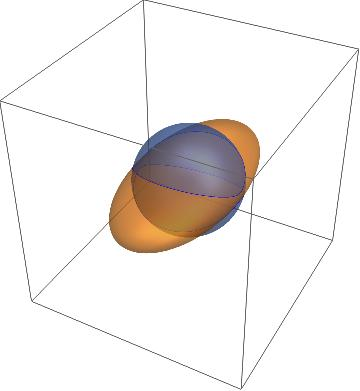
\includegraphics[width=.35\textwidth]{figures/sphere-ellipsoid-inters.jpg}
		\caption{Intersection of an ellipsoid and a sphere.}
		\label{fig:sphere-ellipsoid-inters}
	\end{figure}
	\begin{figure}[H]
		\centering
		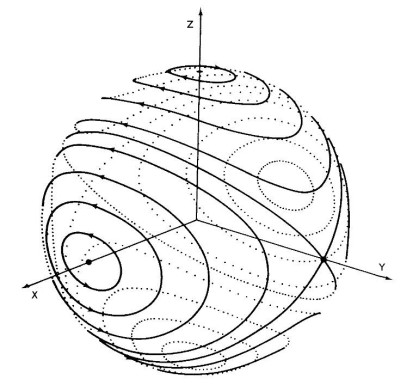
\includegraphics[width=.35\textwidth]{figures/rigid_body_phase_space.jpg}
		\caption{Some of the possibile trajectories given by $X_h$.}
		\label{fig:rigid_body_phase_space}
	\end{figure}
	On the intersection one can fine two different path with opposite directions (given by $X_h$)
	\begin{eqalign}
		\begin{cases}
			y = \pm \frac{\sqrt{ 2EI_xI_yI_z-R^2I_xI_y+(I_xI_y-I_yI_z)x^2}}{\sqrt{I_xI_z-I_xI_y}}\\
			z = \pm \frac{\sqrt{ 2EI_xI_yI_z-R^2I_xI_z+(I_xI_z-I_yI_z)x^2}}{\sqrt{I_xI_y-I_xI_z}}
		\end{cases}
	\end{eqalign}
	which may assume complex values if the sphere and the ellipsoid does not intersect. Then we just have to derive the equation of motion for the $x$ coordinate:
	\begin{eqalign}
		\der{x}{t} = \frac{I_y-I_z}{I_yI_z}yz = \sqrt{\alpha+\beta x^2 + \gamma x^4}
	\end{eqalign}
	with $\alpha, \beta, \gamma$ constants. This gives an elliptic integral
	\begin{eqalign}
		\int_{t_0}^t dt = \int_{x(t_0)}^x \frac{1}{\sqrt{\alpha+\beta x^2 + \gamma x^4}}\,dx
	\end{eqalign}
	which can be solved using complex analysis as we done for the Kepler's problem.\\
	We can also consider Euler's equations for the motion of a rigid body in the frame attached to the rotating body:
	\begin{eqalign}
	\label{eq:euler_eq_rigid_body}
		\der{L}{t} + \omega\times L = M
	\end{eqalign}
	where $L=I(\omega)$ is  the angular momentum, $M$ embodies the external forces, and $I$ is the ineritial tensor
	\begin{eqalign}
		I = \int_{\R^3} \rho(\vec x)\big(|\vec x|^2\id(\bullet)-(\vec x, \bullet)_{\R^3}\tens \vec x\big)\,d^3x \in (\R^3)^*\tens \R^3 \iso \Hom(\R^3 \to \R^3)
	\end{eqalign}
	for some density function $\rho : \R^3\to\R_+$. Thanks to the symmetry of $I$ respect to the scalar product $(\bullet, \bullet)_{\R^3}$, the angular momentum $L=I(\omega)$ can be diagonalized in the frame of principal inertia axis
	\begin{eqalign}
		L = I(\omega) = (I_x\omega_x, I_y\omega_y, I_z\omega_z)
	\end{eqalign}
	giving the eigenvalues $I_x, I_y, I_z$. Equation of motion~\eqref{eq:euler_eq_rigid_body} then can be solved for eigenvectors $\omega_x, \omega_y, \omega_z$ giving
	\begin{eqalign}
		\der{L}{t} = -\omega\times L + M = - \left(\der{L_x}{I_x}, \der{L_y}{I_x}, \der{L_z}{I_z} \right)\times L + M
	\end{eqalign}
	i.e.
	\begin{eqalign}
		\der{L_x}{t} &= (I_z^{-1} - I_y^{-1})L_yL_z+M_x\\
		\der{L_y}{t} &= (I_x^{-1} - I_z^{-1})L_zL_x+M_y\\
		\der{L_z}{t} &= (I_y^{-1} - I_x^{-1})L_xL_y+M_z
	\end{eqalign}
	If we consider the case $M=\vec 0$ then previous equations describe the e.o.m. of the angular momentum for a free rigid body.  In such case, if we consider again Figure~\ref{fig:rigid_body_phase_space}, we can represent the vector $L$ as a vector attached to the center of the sphere whose tip follows the trajectory given by the intersection.  
\end{example}

\section{Poisson cohomology}
\label{sec:poiss_coh}

It should be clear by now that Poisson geometry is closely related to symplectic geometry. There is a strict correspondence between the data of a symplectic structure and those of a Poisson one, and the same with constructions. In particular we have in both contexts the notion of an Hamiltonian vector field, and then a stronger one, called respectively symplectic and Poisson vector fields, which are Hamiltonian fields whose flow preserve the structure.

 \begin{center}
 	\begin{tabular}{c|c}
 		\textbf{Symplectic geometry} & \textbf{Poisson geometry}\\[1ex]
 		\hline
 		$\omega \in \Omega^2(M)$ & $\Pi \in \Lambda^2(M)$\\[1.5ex]
 		$d\omega = 0$ & $[\Pi,\Pi] = 0$\\[1.5ex]
 		non-degeneracy & \textcolor{gray}{(nothing)}\\[1.5ex]
 		Hamiltonian v.f.: & Hamiltonian v.f.:\\
 		$X_f = (\omega^\sharp)^{-1}(df)$ & $X_f = \Pi^\sharp(df)$\\[1.5ex]
 		symplectic v.f.: & Poisson v.f.:\\
 		$\Lie{X}\omega = 0$ & $\Lie{X}\Pi = 0$
 	\end{tabular}
 \end{center}

We clearly see a parallel between Poisson vs. Hamiltonian fields and symplectic vs. Hamiltonian fields. Indeed, the symplectic definitions are identical to the Poisson analogous. We've already analyzed the relationship between Hamiltonian and symplectic fields: we've seen they stand in the same relationship as closed and exact forms of the ambient manifold are (Remark~\ref{rmk:symp_cohomology_is_dr_cohomology}), hence the first de Rham cohomology already gives which obstructions might prevent a symplectic field from being Hamiltonian. In the same spirit, we wish now to construct a cohomology theory which could encode the obstructions preventing a Poisson field from being Hamiltonian, that is, Poisson cohomology.

To start, we look for a coboundary map in the definitions of Poisson and Hamiltonian fields. A Poisson vector field is defined by the condition
\begin{eqalign}
	\Lie{X}\Pi = 0
\end{eqalign}
and an Hamiltonian vector field by
\begin{eqalign}
	X = \Pi^\sharp(df)\ \text{for some $f \in \Cinfty(M)$}.
\end{eqalign}
We leverage the inductive definition of the Schouten--Nijenhuis bracket to convert the Lie derivative along $X$ in a bracket:
\begin{eqalign}
	[\Pi, X] = 0
\end{eqalign}
and in the same vein, we can express $\Pi^\sharp(df)$ as a bracket:
\begin{eqalign}
	\Pi^\sharp(df) &= \frac12 \Pi^{ij} \partial_j f\, \partial_i - \frac12 \Pi^{ij} \partial_i f\, \partial_j\\
		&= \frac12 \Pi^{ij} \partial_i \wedge [f, \partial_j] - \frac12 [f,\Pi^{ij}\partial_i] \wedge \partial_j\\
		&= [\frac12 \Pi^{ij}\partial_i \wedge \partial_j, f]\\
		&= [\Pi, f].
\end{eqalign}
Hence we might guess our coboundary map to be $d_\Pi := [\Pi, \bullet]$. To be such a map, it must square to zero:

\begin{lemma}
\label{lemma:poisson_coboundary}
	Let $\Pi \in \Lambda^2(M)$ be a Poisson tensor. Then
	\begin{eqalign}
		[\Pi,[\Pi,A]] = 0, \quad \forall A \in \Lambda^k(M).
	\end{eqalign}
\end{lemma}
\begin{proof}
	Using the graded Jacobi identity (Exercise~\ref{ex:graded_jacobi}), and recalling $|\Pi|=2$:
	\begin{eqalign}
		(-1)^{k-1}\,[\Pi,[\Pi,A]]-[\Pi,[A,\Pi]]+(-1)^{k-1}\,[A,\underbrace{[\Pi,\Pi]}_{=0}] &= 0\\
		2(-1)^{k-1}\,[\Pi,[\Pi,A]] &= 0 \comment{by graded skew-symmetry}\\
		[\Pi,[\Pi,A]] &= 0.
	\end{eqalign}
\end{proof}

The cochain complex arising from these coboundaries is called the \textbf{Poisson complex}:
\begin{diagram}
	\ldots \arrow{r}{d_\Pi} \&\Lambda^p(M) \arrow{r}{d_\Pi} \& \Lambda^{p+1}(M) \arrow{r}{d_\Pi} \& \ldots
\end{diagram} 

\begin{definition}
	The $r$-th Poisson cohomology of $(M, \Pi)$ is
	\begin{eqalign}
		H^r_\Pi (M) = \ker d^{(r)}_\Pi / \im d^{(r-1)}_\Pi
	\end{eqalign}
	where $d^{(k)}_\Pi$ denotes $d_\Pi : \Lambda^k(M) \to \Lambda^{k+1}(M)$.
\end{definition}

\begin{example}
	For the trivial Poisson tensor $\Pi = 0$, $H^r_\Pi \iso \Lambda^r(M)$. Notice that the Poisson cohomology can be infinite dimensional. This is not the case of the de Rham cohomology, which under loose (satisfied) assuptions is finite dimensional. 
\end{example}

\begin{example}
	In the symplectic case ($\Pi$ non-degenerate), then $\Pi^\sharp$ induces an identification of $\Omega^\bullet$ with $\Lambda^\bullet$, which commutes with the de Rham's and Poisson differentials:
	\begin{diagram}
		\ldots \arrow{r}{d} \& \Omega^p(M) \arrow{d}{\Pi^\sharp} \arrow{r}{d} \& \Omega^{p+1}(M) \arrow{d}{\Pi^\sharp} \arrow{r}{d} \& \ldots\\
		\ldots \arrow{r}{d_\Pi} \& \Lambda^p(M) \arrow{r}{d_\Pi} \& \Lambda^{p+1}(M) \arrow{r}{d_\Pi} \& \ldots
	\end{diagram}
	This is called, in homological algebra, a \textbf{(co)chain isomorphism} and implies that the cohomologies arising from the two complexes are naturally isomorphic. Thus, \textbf{in the symplectic case, Poisson cohomology coincides with de Rham cohomology}, as expected.
\end{example}

\begin{example}
	Consider the Lie--Poisson structure on $\lalg^*$. For this case, it turns out
	\begin{eqalign}
		H^k_\Pi(\lalg^*) \iso H^k_L(\lalg) \tens \Cas(\lalg^*) \iso H^k_L(\lalg) \tens \Cinfty(\lalg^*)^G
	\end{eqalign}
	where
	\begin{enumerate}
		\item $H^k_L(\lalg)$ is the $k$-th Lie cohomology\footnotemark\ of $\lalg$,
		\item $\Cas(\lalg^*)$ is the space of Casimir functions on $\lalg^*$, i.e. functions constant on symplectic leaves (coadjoint orbits),
		\item $\Cinfty(\lalg^*)^G$ is the space of functions invariant w.r.t. the coadjoint $G$-action.
	\end{enumerate}
	\footnotetext{The \textbf{Lie cohomology} of a (real) Lie algebra $\lalg$ of finite dimension $n$ is defined from the Chevalley--Eilenberg complex, whose objects are the $k$-th exterior powers of $\lalg^*$ and the coboundary maps ${d_L^{(k)} : \wedge^k \lalg^* \to \wedge^{k+1}\lalg^*}$ are given by:
	\begin{eqalign}
		(d_L\alpha)(X_0, \ldots, X_k) = \sum_{0 \leq i \leq j \leq n} (-1)^{i+j} \alpha([X_i, X_j], X_2, \ldots, \hat{X_i}, \ldots, \hat{X_j}, \ldots, X_k).
	\end{eqalign}
	Alternatively, $d_L$ can be defined axiomatically and inductively from its values on the $1$-$\lalg$-forms}
\end{example}

\subsection{Meaning of the Poisson cohomologies}
We now set to interpret the Poisson cohomologies of a given manifold $(M, \Pi)$. Let's start with the zeroth cohomology: it is the space of all $f \in \Cinfty(M)$ such that $[\Pi, f] = 0$. As we've shown in a previous calculation, this is the same as saying $\{f,\bullet\} = 0$, meaning
\begin{eqalign}
	H_\Pi^0(M) = \Cas(M) =\text{Casimir functions}.
\end{eqalign}

Next, the interpretation of the first cohomology was our motivational example:
\begin{eqalign}
	H_\Pi^1(M) = \frac{\text{Poisson vector fields}}{\text{Hamiltonian vector fields}}
\end{eqalign}

Finally, both $2$-cocycles and $2$-boundaries assume meaning in the context of \textbf{Poisson infinitesimal deformations}. A \emph{deformation} of $\Pi$ is another Poisson tensor $\Pi'$ obtained by adding a bivector $\Delta = \Pi' - \Pi$. An \emph{infinitesimal deformation} is a deformation ``up to the first-order'', i.e. it is of the form $\Pi + \varepsilon \Delta$ for $\varepsilon > 0$, but we only require $[\Pi', \Pi'] = O(\varepsilon^2)$, hence
\begin{eqalign}
	[\Pi + \varepsilon \Delta, \Pi + \varepsilon\Delta] - [\Pi,&\Pi] = 2\varepsilon[\Pi,\Delta] + \varepsilon^2[\Delta, \Delta] = O(\varepsilon^2) \iff [\Pi, \Delta] = 0.
\end{eqalign}
From a cohomological point of view, this latter condition might be better expressed as $\Delta \in \ker d_\Pi^{(2)}$.

However, a deformation of $\Pi$ can be also given through a local diffeomorphism, like the flow of a vector field $X$. In this way, the deformed Poisson tensor is\footnote{Notice higher order terms here vanish completely since $\Lie{X}^2\Pi = [\Pi, [\Pi, X]] = 0$ by Lemma~\ref{lemma:poisson_coboundary}.}
\begin{eqalign}
	(\phi_\varepsilon)_* \Pi = \Pi + \varepsilon \Lie{X}\Pi = \Pi + \varepsilon (\underbrace{\Lie{X}\Pi}_\Delta).
\end{eqalign}
As we see in the above expression, this second case can be seen as a particular form of the first one, in fact a ``trivial'' one: diffeomorphisms are just changes of coordinates, and they don't really change the Poisson structure. Notice moreover that $\Delta$ is given above as the Taylor expansion of $[\Pi, X]$, hence $\Delta \in \im d^{(1)}_\Pi$.

Therefore we reach an interpretation for $H_\Pi^2(M)$: \textbf{it is the space of non-trivial infinitesimal deformations of $\Pi$}:
\begin{eqalign}
	H^2_\Pi(M) = \frac{\text{infinitesimal deformations of $\Pi$}}{\text{trivial infinitesimal deformations of $\Pi$}}
\end{eqalign}

\begin{remark}
	The fact that first-order infinitesimal deformations exist does not imply a full-blown deformation exist! However, if it does, then it determines completely the coefficients of such deformation.
\end{remark}

Higher cohomologies do not have, in general, an enlightening interpretation in terms of geometrical property of the manifold, but the general cohomological interpretation remains valid: they represent obstructions to ``deformations'' of higher orders.

\begin{example}
	Let $M=S^2$ equipped with the usual symplectic structure (the area form pulled back from the volume form of $\R^3$). We know then $H^2_\Pi(S^2) \iso H^2_{dR}(S^2) =\langle \omega \rangle \iso \R$ because, up to rescaling, there's only one volume closed form which is not exact.

	Indeed, any infinitesimal deformation has the form $\Pi + \varepsilon \Pi = (1+\varepsilon)\Pi$, i.e. a rescaling. But the diffeomorphism between a sphere of radius $1$ and one of radius $1+\varepsilon$ is not a symplectomorphism since it is not area preserving, hence they are all different Poisson structures.
\end{example}

\begin{example}[{Ginzburg, \cite[Proposition 4.19]{ciccoli2006lectures}}]
	Consider $(\R^2, \Pi_0 = (x^2+y^2)\,\partial_x \wedge \partial_y)$. The Poisson tensor has only one singular point, the origin. Therefore the symplectic foliation is composed of two leaves: the origin and the rest of $\R^2$. The Poisson cohomology is
	\begin{eqalign}
		H_\Pi^0(\R^2, \Pi_0) &= \R \comment{(since constant functions on the symp. leaves are Casimir)}\\
		H_\Pi^1(\R^2, \Pi_0) &= \mathrm{span}_\R \{ x\,\partial_x + y\,\partial_y,\; y\,\partial_x - x\,\partial_y \}\\
		H_\Pi^2(\R^2, \Pi_0) &= \mathrm{span}_\R \{ \partial_x \wedge \partial_y,\; \Pi_0 \}.
	\end{eqalign}
	See the reference for explicit computations.
\end{example}

\end{document}